Hooke's Law is a physical principle that states that a spring stretched (extended) or compressed by some distance produces a restoring force which is directly proportional to said distance. Mathematically, if an extension $x$ is accompanied by a restoring force $F$ then they are related by the equation
%
\beq \label{hookes_law}
    F = k \, x
\eeq
%
where $k$ is the Spring Constant.

\section*{Experimental Setup}

    \tikzsetnextfilename{single_spring}

\begin{center}
    \begin{tikzpicture}

        
% Define styles that will automatically draw the spring and slanting line platform objects
\tikzstyle{spring1}=[thick, decorate, decoration={aspect=0.5, segment length=2mm, amplitude=2mm, coil}]
\tikzstyle{spring2}=[thick, decorate, decoration={aspect=0.5, segment length=3mm, amplitude=2mm, coil}]

\tikzstyle{platform}=[fill, pattern=north east lines, draw=none]

% Define a 'newdrawing' that corresponds to the weight box
\newdrawing{\weight}{
    \def\hw{0.25}
    \draw (-\hw, 0) rectangle (\hw, {-2 * \hw}) node [midway] {$m$};        % Note: the use of [midway] to place the label midway between the starting and ending points of the rectangle
}

\def\ph{0.25}       % height of the slanted line rectangle that constitutes a platform


        \def\l{2}           % Length of spring
        \def\hw{0.75}

        \draw [platform] (-\hw,\l) rectangle (\hw,{\l + \ph});
        \draw [very thick] (-\hw,\l) -- (\hw,\l);       % Thick line underneath platform to which the spring is attached
        \draw [spring1] (0,\l) -- (0,0) node [midway, right=7] {$k$};

        \weight[]           % Draw the weight object using the command generated by the newdrawing macro

    \end{tikzpicture}
\end{center}


    The weight of the mass attached to the bottom of the spring provides the force necessary to stretch it. The extension of the spring is measured using the pointer attached to the mass hanger. The position of the pointer is read off from the ruler placed behind the pointer.

\section*{Balancing Forces}

    If a weight is attached to an initially unextended spring the force applied by the weight is unbalanced and causes the spring to begin stretching (extending). As the extension of the spring increases it produces a restoring force given by \eqref{hookes_law} whose purpose is to oppose the stretching and return the spring to its initial unstretched condition. When the spring has extended enough the restoring force exactly balances the weight of the mass and the system achieves equilibrium.

    This is demonstrated by a free-body diagram of the mass where the only two forces acting upon it are its weight and the restoring force exerted by the spring.

    \tikzsetnextfilename{single_fbd}

\begin{center}
    \begin{tikzpicture}

        
% Define styles that will automatically draw the spring and slanting line platform objects
\tikzstyle{spring1}=[thick, decorate, decoration={aspect=0.5, segment length=2mm, amplitude=2mm, coil}]
\tikzstyle{spring2}=[thick, decorate, decoration={aspect=0.5, segment length=3mm, amplitude=2mm, coil}]

\tikzstyle{platform}=[fill, pattern=north east lines, draw=none]

% Define a 'newdrawing' that corresponds to the weight box
\newdrawing{\weight}{
    \def\hw{0.25}
    \draw (-\hw, 0) rectangle (\hw, {-2 * \hw}) node [midway] {$m$};        % Note: the use of [midway] to place the label midway between the starting and ending points of the rectangle
}

\def\ph{0.25}       % height of the slanted line rectangle that constitutes a platform


        \def\l{\hww+\lv}           % Length of each arrow

        % \draw (\hw, \hw) rectangle (-\hw, -\hw) node [midway] {$m$};
        \weight[yshift=\hww]
        \draw [->, thick] (0,\hww) -- (0,\l) node [above] {$F = k x$};
        \draw [->, thick] (0,-\hww) -- (0,{-\hww-\lv}) node [below] {$W = m g$};

    \end{tikzpicture}
\end{center}


    Therefore at equilibrium (when the mass-spring system is at rest) the two forces must be balanced and so
    \beqs \label{mgkx}
        F - mg &= 0\\
        \imply kx - mg &= 0\\
        \imply kx &= mg\\
        \imply x &= \frac{g}{k} m\\
    \eeqs

    The final equation gives the relation between the mass attached to the string and the extension it produces.

\setcounter{section}{0}
\section{Single Spring}

    Using equation \eqref{mgkx} one can calculate the spring constant $k$ of a spring my performing an experiment where one varies the attached mass $m$ and measures the corresponding extension $x$. The slope of the graph of $x$ vs. $m$ is then given by $g / k$.

\section{Springs in parallel}

    A mass can be suspended from two springs in parallel by connecting the bottoms of the two springs by a pole and suspending the mass from its center, as shown in the diagram below.

    \tikzsetnextfilename{parallel_springs}

\begin{center}
    \begin{tikzpicture}

        
% Define styles that will automatically draw the spring and slanting line platform objects
\tikzstyle{spring1}=[thick, decorate, decoration={aspect=0.5, segment length=2mm, amplitude=2mm, coil}]
\tikzstyle{spring2}=[thick, decorate, decoration={aspect=0.5, segment length=3mm, amplitude=2mm, coil}]

\tikzstyle{platform}=[fill, pattern=north east lines, draw=none]

% Define a 'newdrawing' that corresponds to the weight box
\newdrawing{\weight}{
    \def\hw{0.25}
    \draw (-\hw, 0) rectangle (\hw, {-2 * \hw}) node [midway] {$m$};        % Note: the use of [midway] to place the label midway between the starting and ending points of the rectangle
}

\def\ph{0.25}       % height of the slanted line rectangle that constitutes a platform


        \def\l{2}           % Length of spring
        \def\hw{1.5}
        \def\hws{1}

        \draw [platform] (-\hw,\l) rectangle (\hw,{\l+\ph});    % Using the [platform] modifier sets the fill pattern for the rectangle
        \draw [very thick] (-\hw,\l) -- (\hw,\l);       % Thick line underneath platform to which the spring is attached

        \draw [spring1] (-\hws,\l) -- (-\hws,0);
        \draw [spring2] (\hws,\l) -- (\hws,0);

        \draw [very thick] (-\hw, 0) -- (\hw, 0);
        \draw (0,0) -- (0,-0.25);

        \weight[yshift=-0.25]           % Draw the weight object using the command generated by the newdrawing macro

    \end{tikzpicture}
\end{center}


    The weight of the mass causes both springs to be extended by the same amount $x$ since they are connected by means of the pole. The two springs are essentially responding to the weight of the mass by extending and applying a restoring force. Thus together they are behaving as a single spring would behave.

    The question is: What is the \textit{effective} spring constant of the two parallel springs? That is, for what value of the spring constant would a \textbf{single} spring have the same effect as the two springs in parallel.

    Let the two springs have spring constants $k_1$ and $k_2$. Let the effective spring constant (of the equivalent single spring) be $k$. If the application of mass $m$ to the system produces an extension $x$ we can use \eqref{mgkx} to relate $x$ to $m$ using the spring constants. For the single spring case the equation is straight-forward, it is simply \eqref{mgkx}.

    For the springs in parallel we draw a free-body diagram and equate the upward and downward forces.

    \eline[0.5]
    \tikzsetnextfilename{parallel_fbd}

\begin{center}
    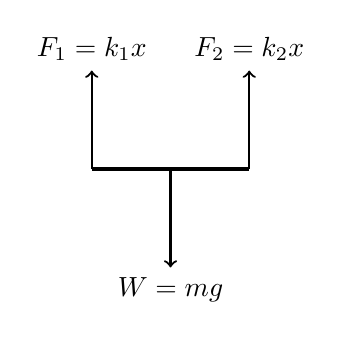
\begin{tikzpicture}

        \def\hws{1}
        \def\l{1.25}

        \draw [very thick] (-\hws, 0) -- (\hws, 0);

        \draw [->, thick] (0,0) -- (0,-\l) node [below] {$W = m g$};
        \draw [->, thick] (-\hws, 0) -- (-\hws, \l) node [above] {$F_1 = k_1 x$};
        \draw [->, thick] (\hws, 0) -- (\hws, \l) node [above] {$F_2 = k_2 x$};

    \end{tikzpicture}
\end{center}


    Since the two springs in parallel have the same extension $x$ we have
    \beq \label{parallel}
        k_1 x + k_2 x = mg
    \eeq

    Since the parallel spring system and the effective single spring are by definition equivalent we can use \eqref{mgkx} to substitute for $mg$ in \eqref{parallel} giving us
    %
    \beqc
        k x = m g = k_1 x + k_2 x\\
        \imply k x = (k_1 + k_2) x\\
        \imply k = k_1 + k_2
    \eeqc

    Therefore the \textit{effective} spring constant of two springs in parallel is simply the sum of their individual spring constants. This basically indicates that it is \textbf{harder} to stretch two springs in parallel than it is to stretch either one by itself.


\section{Springs in series}

    A mass can be suspended from two springs in series by connecting the bottom of upper spring to the top of the lower spring, as shown in the diagram below.

    \tikzsetnextfilename{series_springs}

\begin{center}
    \begin{tikzpicture}

        
% Define styles that will automatically draw the spring and slanting line platform objects
\tikzstyle{spring1}=[thick, decorate, decoration={aspect=0.5, segment length=2mm, amplitude=2mm, coil}]
\tikzstyle{spring2}=[thick, decorate, decoration={aspect=0.5, segment length=3mm, amplitude=2mm, coil}]

\tikzstyle{platform}=[fill, pattern=north east lines, draw=none]

% Define a 'newdrawing' that corresponds to the weight box
\newdrawing{\weight}{
    \def\hw{0.25}
    \draw (-\hw, 0) rectangle (\hw, {-2 * \hw}) node [midway] {$m$};        % Note: the use of [midway] to place the label midway between the starting and ending points of the rectangle
}

\def\ph{0.25}       % height of the slanted line rectangle that constitutes a platform


        \def\la{2}           % Length of spring
        \def\lb{4}
        \def\hw{0.75}

        \draw [platform] (-\hw,\lb) rectangle (\hw,{\lb + \ph});
        \draw [very thick] (-\hw,\lb) -- (\hw,\lb);       % Thick line underneath platform to which the spring is attached

        \draw [spring2] (0,{\la + 0.2}) -- (0,\lb) node [midway, right=10] {$k_2$};

        % Draw a line with a small circle in the middle to show the connection between the two springs
        \draw (0,\la) -- (0,{\la + 0.2});
        \draw [fill=black] (0,{\la + 0.1}) circle [radius=0.05];

        \draw [spring1] (0,\la) -- (0,0) node [midway, right=10] {$k_1$};

        \weight[]

    \end{tikzpicture}
\end{center}


    The weight of the mass causes the lower spring to extend which in turn applies a force on the upper spring causing it to extend as well. The force experienced by both springs is equal to the weight of the object. This can be demonstrated by drawing free-body diagrams (below) of the point where the mass is attached and the point where the two springs meet. At equilibrium both of these points are stationary and so the net force acting on them must be zero.

    \begin{minipage}{0.5\textwidth}
        \tikzsetnextfilename{series_fbd1}

\begin{center}
    \begin{tikzpicture}

        
% Define styles that will automatically draw the spring and slanting line platform objects
\tikzstyle{spring1}=[thick, decorate, decoration={aspect=0.5, segment length=2mm, amplitude=2mm, coil}]
\tikzstyle{spring2}=[thick, decorate, decoration={aspect=0.5, segment length=3mm, amplitude=2mm, coil}]

\tikzstyle{platform}=[fill, pattern=north east lines, draw=none]

% Define a 'newdrawing' that corresponds to the weight box
\newdrawing{\weight}{
    \def\hw{0.25}
    \draw (-\hw, 0) rectangle (\hw, {-2 * \hw}) node [midway] {$m$};        % Note: the use of [midway] to place the label midway between the starting and ending points of the rectangle
}

\def\ph{0.25}       % height of the slanted line rectangle that constitutes a platform


        \def\l{\lv + \hww}

        \weight[yshift=\hww]
        \draw [->, thick] (0,\hww) -- (0, \l) node [above] {$F_1 = k_1 x_1$};
        \draw [->, thick] (0, -\hww) -- (0, {-\lv -\hww}) node [below] {$W = m g$};

    \end{tikzpicture}
\end{center}

    \end{minipage}
    \begin{minipage}{0.5\textwidth}
        \tikzsetnextfilename{series_fbd2}

\begin{center}
    \begin{tikzpicture}

        
% Define styles that will automatically draw the spring and slanting line platform objects
\tikzstyle{spring1}=[thick, decorate, decoration={aspect=0.5, segment length=2mm, amplitude=2mm, coil}]
\tikzstyle{spring2}=[thick, decorate, decoration={aspect=0.5, segment length=3mm, amplitude=2mm, coil}]

\tikzstyle{platform}=[fill, pattern=north east lines, draw=none]

% Define a 'newdrawing' that corresponds to the weight box
\newdrawing{\weight}{
    \def\hw{0.25}
    \draw (-\hw, 0) rectangle (\hw, {-2 * \hw}) node [midway] {$m$};        % Note: the use of [midway] to place the label midway between the starting and ending points of the rectangle
}

\def\ph{0.25}       % height of the slanted line rectangle that constitutes a platform


        \draw [fill=black] (0,0) circle [radius=0.05];

        \draw [->, thick] (0,0) -- (0,\lv) node [above] {$F_2 = k_2 x_2$};
        \draw [->, thick] (0,0) -- (0,-\lv) node [below] {$F_1 = k_1 x_1$};

    \end{tikzpicture}
\end{center}

    \end{minipage}

    \eline[0.5]
    Equating the upward and downward forces gives us $F_1 = W$ and $F_2 = F_1 = W$. Therefore in the series configuration each spring experiences the same force as the lowest spring. Each spring will response to this force with a different extension $x_1$ and $x_2$ since they have different spring constants $k_1$ and $k_2$. The net extension of the two-spring system is then the sum of the extensions of each individual spring: $x = x_1 + x_2$. We can now calculate the effective spring constant $k$ (a single spring with the same extension as the two springs in series) using \eqref{hookes_law} which tells us that $\displaystyle x = \frac{F}{k}$.
    %
    \beqc
        x = x_1 + x_2\\
        \imply \frac{F}{k} = \frac{F_1}{k_1} + \frac{F_2}{k_2}\\
        \imply \frac{W}{k} = \frac{W}{k_1} + \frac{W}{k_2}\\
        \imply \frac{1}{k} = \frac{1}{k_1} + \frac{1}{k_2}
    \eeqc

    Therefore the \textit{effective} spring constant of two springs in series is the inverse of the sum of the inverse of their individual spring constants. This basically indicates that it is \textbf{easier} to stretch two springs in series than it is to stretch either one by itself.


\section{Oscillating Spring}

    When a spring is deformed (either stretched or compressed) a restoring force is set up which wants to bring the spring back to its original position. In a spring-mass system this means works must always be done on the mass to move it away from the mean/equilibrium position. Equivalently a mass gains Elastic Potential Energy whenever it is displaced from the equilibrium position.

    If we stretch a spring-mass system and release it from rest we basically store Elastic Potential Energy inside it. After being released the restoring force pulls the mass back towards the equilibrium position. As it moves back to this position the mass loses Elastic P.E. but due to the conservation of energy gains Kinetic Energy. When the mass returns to the equilibrium position its Elastic P.E. is zero but all of its initial energy is now in the form of K.E. Consequently the object is moving at maximum speed and cannot remain at the equilibrium position.

    The mass moves past the equilibrium position and now once again a restoring force is pulling it back. The mass loses K.E. and gains Elastic P.E. It comes to rest when all of the K.E. has been converted to P.E. and it finds itself at the same distance from the equilibrium as when it started but in the opposite direction.

    Once again the mass starts its journey back to the equilibrium position and once again it is unable to remain there due to K.E. As a result the mass is forced to continuously move back and forth, or in other words oscillate.

    Every oscillating system has a Time Period, which is the time it takes for the system to completely one cycle, one sequence of motions which is then repeated endlessly. The Time Period, T, of a mass-spring system is given by:
    %
    \beq
        T = 2 \pi \sqrt{\frac{m}{k}}
    \eeq
